\documentclass[12pt]{article}
\usepackage{graphicx,import}
\usepackage[svgnames]{xcolor} 
\usepackage{fancyhdr}
\usepackage{subfig}
\usepackage{hyperref}
\usepackage{enumitem}
\usepackage{cite}
\usepackage[many]{tcolorbox}
\usepackage{listings }
\usepackage[a4paper, total={6in, 8in} , bottom = 25mm , top = 25mm, headheight = 1.25cm , includehead,includefoot,heightrounded ]{geometry}
\usepackage{afterpage}
\usepackage{amssymb}
\usepackage{pdflscape}
\usepackage{gensymb}
\usepackage{textcomp}
\usepackage{tikz,pgfplots}
\usepackage{xecolor}
\usepackage{rotating}
\usepackage{pdfpages}
\usepackage[Kashida]{xepersian}
\usepackage[T1]{fontenc}
\usepackage{tikz}
\usepackage[utf8]{inputenc}
\usepackage{PTSerif} 
\usepackage{seqsplit}

\usepackage[edges]{forest}

\usepackage{listings}
\usepackage{xcolor}

\hypersetup{
	colorlinks   = true, %Colours links instead of ugly boxes
	urlcolor     = blue, %Colour for external hyperlinks
	linkcolor    = blue, %Colour of internal links
	citecolor   = red %Colour of citations
}
 
\definecolor{codegreen}{rgb}{0,0.6,0}
\definecolor{codegray}{rgb}{0.5,0.5,0.5}
\definecolor{codepurple}{rgb}{0.58,0,0.82}
\definecolor{backcolour}{rgb}{0.95,0.95,0.92}
 
\NewDocumentCommand{\codeword}{v}{
\texttt{\textcolor{blue}{#1}}
}
\lstset{language=java,keywordstyle={\bfseries \color{blue}}}

\lstdefinestyle{mystyle}{
    backgroundcolor=\color{backcolour},   
    commentstyle=\color{codegreen},
    keywordstyle=\color{magenta},
    numberstyle=\tiny\color{codegray},
    stringstyle=\color{codepurple},
    basicstyle=\ttfamily\normalsize,
    breakatwhitespace=false,         
    breaklines=true,                 
    captionpos=b,                    
    keepspaces=true,                 
    numbers=left,                    
    numbersep=5pt,                  
    showspaces=false,                
    showstringspaces=false,
    showtabs=false,                  
    tabsize=2
}

\lstset{style=mystyle}

\settextfont[Scale=1.2 ,BoldFont={Bahij Nazanin-Bold.ttf} , ItalicFont = {IRNazaninIranic.ttf}]{Bahij Nazanin-Regular.ttf}
\setlatintextfont[Scale = 1.0]{Garamond}
\DefaultMathsDigits 
\DeclareMathSizes{11}{19}{13}{9} 
%\DeclareMathSizes{12}{14.4}{8}{9}





\newenvironment{changemargin}[2]{%
\begin{list}{}{%
\setlength{\topsep}{0pt}%
\setlength{\leftmargin}{#1}%
\setlength{\rightmargin}{#2}%
\setlength{\listparindent}{\parindent}%
\setlength{\itemindent}{\parindent}%
\setlength{\parsep}{\parskip}%
}%
\item[]}{\end{list}}


\definecolor{foldercolor}{RGB}{124,166,198}

\tikzset{pics/folder/.style={code={%
    \node[inner sep=0pt, minimum size=#1](-foldericon){};
    \node[folder style, inner sep=0pt, minimum width=0.3*#1, minimum height=0.6*#1, above right, xshift=0.05*#1] at (-foldericon.west){};
    \node[folder style, inner sep=0pt, minimum size=#1] at (-foldericon.center){};}
    },
    pics/folder/.default={20pt},
    folder style/.style={draw=foldercolor!80!black,top color=foldercolor!40,bottom color=foldercolor}
}

\forestset{is file/.style={edge path'/.expanded={%
        ([xshift=\forestregister{folder indent}]!u.parent anchor) |- (.child anchor)},
        inner sep=1pt},
    this folder size/.style={edge path'/.expanded={%
        ([xshift=\forestregister{folder indent}]!u.parent anchor) |- (.child anchor) pic[solid]{folder=#1}}, inner xsep=0.6*#1},
    folder tree indent/.style={before computing xy={l=#1}},
    folder icons/.style={folder, this folder size=#1, folder tree indent=3*#1},
    folder icons/.default={12pt},
}

\begin{document}


%%% title pages
\begin{titlepage}
\begin{center}
        
\vspace*{0.7cm}


\includegraphics[width=0.4\textwidth]{sharif1.png}\\
\vspace{0.5cm}
\textbf{ \Huge{\emph ‌سیگنال‌ها و سیستم‌ها} }\\
\vspace{0.5cm}
\textbf{ \Large{ تمرین دوم} }
\vspace{0.2cm}
       
 
      \large \textbf{دانشکده مهندسی کامپیوتر}\\\vspace{0.2cm}
    \large   دانشگاه صنعتی شریف\\\vspace{0.2cm}
       \large   ﻧﯿﻢ سال دوم 00-99 \\\vspace{0.2cm}
      \noindent\rule[1ex]{\linewidth}{1pt}
استاد:\\
    \textbf{{جناب آقای دکتر منظوری شلمانی}}


    \vspace{0.15cm}
نام و نام خانوادگی:\\

       
    \textbf{{امیرمهدی نامجو - 97107212}}
\end{center}
\end{titlepage}
%%% title pages


%%% header of pages
\newpage
\pagestyle{fancy}
\fancyhf{}
\fancyfoot{}
\cfoot{\thepage}
\chead{تمرین دوم}
\rhead{
\includegraphics[width=0.1\textwidth]{sharif.png}}
\lhead{امیرمهدی نامجو}
%%% header of pages

\KashidaOff

\section{سوال اول}


\begin{enumerate}[label = \Alph*)]
	
	\item
	$x(t) = e^{3 |t|}$
	
	$$\mathcal{L}(x(t)) = \int_{-\infty}^{\infty} e^{3 |t|} e^{-s t} dt = \int_{0}^{\infty} e^{(3-s)t} dt+ \int_{-\infty}^{0} e^{(-3-s)t} dt$$
	
	$$= \frac{e^{(3-s)t}}{3-s}|_{0}^{\infty} + \frac{e^{(-3-s)t}}{-3-s}|_{-\infty}^{0} = \frac{1}{s-3} + \frac{-1}{s+3} = \frac{6}{s^2 - 9}$$
	
	با این حال باید توجه کرد که ناحیه همگرایی عامل اول برای $Re(s)>3$ بوده و ناحیه همگرایی عامل دوم جمع
	$-3 - Re(s) > 0 \rightarrow Re(s)<-3$
	است. در نتیجه این عبارت تبدیل لاپلاس ندارد چون ناحیه همگرایی کلی آن تهی است.
	
	\item
	$x(t) = e^{-3 |t|}$
	
		$$\mathcal{L}(x(t)) = \int_{-\infty}^{\infty} e^{-3 |t|} e^{-s t} dt = \int_{0}^{\infty} e^{(-3-s)t} dt+ \int_{-\infty}^{0} e^{(3-s)t} dt$$
	
	$$= \frac{e^{(-3-s)t}}{-3-s}|_{0}^{\infty} + \frac{e^{(3-s)t}}{3-s}|_{-\infty}^{0} = \frac{1}{s+3} + \frac{-1}{s-3} = \frac{6}{s^2 - 9}$$
	
	در این مورد ناحیه همگرایی عامل اول
	 $Re(s) >-3$
	 و برای عامل دوم
	 $Re(s)<3$
	 است که باعث می شود تبدیل لاپلاس درستی با ناحیه همگرایی
	 $-3 < Re(s) < 3$
	 داشته باشیم.
	 
	 
	 
	 \item
	 $$x(t) =e^{(-1 + j) t} \cos(3t) u(t)$$
	
	
	براساس جدول تبدیل لاپلاس:
	
	$$\mathcal{L}(x(t)) = \frac{s - (-1 +j)}{(s - (-1 +j))^2 + 9)} = \frac{s +1 - j}{9 + s^2 + (2-2j)s - 2j}$$
	
	برای ناحیه همگرایی عامل کسینوس صرفا نوسان ساز است و تاثیری ندارد. توان موهومی هم ایجاد کننده عوامل نوسان ساز است. تنها توان حقیقی مهم است. با توجه به Right-Side بودن سیگنال، ناحیه همگرایی
	$$Re(s)>-1$$
	است.
	
	
	
\end{enumerate}

\section{سوال دوم}


\begin{enumerate}[label = \Alph*)]
	
	\item
$$
\frac{s}{s^{2}+4}-\frac{5}{s+2}-\frac{1}{s-2} , 0 < Re(s) < 2
$$

برای عبات اول، معکوس آن $\cos(2t)$ خواهد بود. برای عبارت دوم معکوس آن
$5 e^{-2t}$
و برای عبارت سوم معکوس آن
$e^{2t}$
خواهد بود.

با توجه به ناحیه همگرایی متوجه می شویم که عبارت $\cos(2t)$ که ناحیه همگرایی مربوط به صفر را ایجاد کرده باید Right-Sided باشد و در نتیجه $e^{2t}$ هم Right-Sided خواهد بود. اما عبارت $e^{-2t}$ به صورت Left-Sided خواهد بود.


	$$\mathcal{L}^{-1} (X(s))= \cos(2t) u(t) - 5 e^{-2t} u(t) - (- e^{2t} u(-t)) = \cos(2t) u(t) - 5 e^{-2t} u(t) + e^{2t} u(-t)$$


	
	\item
	
	$$
	X(s) =\frac{s+2}{s^{2}+7 s+12} , -4<Re(s)<-3
	$$
	
	$$
	\frac{s+2}{s^{2}+7 s+12} = \frac{2}{s+4} - \frac{1}{s+3}
	$$
	
	
	عامل اصلی تبدیل لاپلاس اولی $e^{-4t}$ و دومی $e^{-3t}$ است. با توجه به ناحیه همگرایی داده شده، برای $-4$ باید Right-Sided داشته باشیم و برای $-3$ عبارت Left-Sided پس:
	
	$$\mathcal{L}^{-1} (X(s))= 2 e^{-4t} u(t) - (- e^{-3t}u(-t)) = 2 e^{-4t} u(t) + e^{-3t}u(-t)$$
	
\end{enumerate}


\section{سوال سوم}

با توجه به شکل داده شده و این که صفر نداریم، یعنی صورت عبارت تبدیل لاپلاس یک عدد ثابت است.  از طرفی با توجه به نقاط قطب ها، عامل مختلط $s^2-2s+2$ و عوامل $s+2$ و $s+1$ وجود دارند. یعنی عبارت اصلی به شکل زیر است:

$$\frac{a}{(s^2-2s+2)(s+2)(s+1)}$$
است. عبارت اول مخرج براساس
$(s - (1+j))(s-(1-j))$
بدست آمده است.

این عبارت را اگر تبدیل به کسر های جزئی کنیم به عبارت زیر می رسیم:

$$X(S)=\frac{a}{10}(\frac{2}{s+1} + \frac{-1}{s+2} + \frac{2  }{(s-1)^2 + 1} + \frac{- s}{(s-1)^2 +1})$$
$$= \frac{a}{10}(\frac{2}{s+1} + \frac{-1}{s+2} + \frac{1  }{(s-1)^2 + 1} + \frac{- (s-1)}{(s-1)^2 +1})$$

با توجه به ناحیه همگرایی داده شده، یعنی عبارت های سینوسی و کسینوسی که از دو بخش آخر بدست می آیند هر دو باید Left-Sided باشند زیرا بخش حقیقی قطب آن ها $1$ است و ناحیه همگرایی در سمت چپ آن اتفاق افتاده است. عبارت مربوط به $s+1$ هم باید Left-Sided باشد و عبارت مربوط به $s+2$ باید Right-Sided باشد.

با توجه به این مسائل و طبق جدول تبدیل لاپلاس داریم:

$$\mathcal{L}^{-1} (X(s)))=\frac{a}{10}\left((-2 e^{-t} u(-t)) + (- e^{-2t}u(t)) + (-e^t \sin(t) u(-t)) + (e^t \cos(t) u(-t))\right)$$


\section{سوال چهارم}

یک فرض منطقی این است که فرض کنیم سیگنال حقیقی باشد. در این صورت

با توجه به این که $-1+i$ جزو قطب هاست پس $-1-i$ هم جزو قطب هاست پس در مخرج
$(s-(-1 + i))(s-(-1 - i)) = s^2 + 2s + 2$
را داریم.

همچنین با توجه به عبارت بالا ناحیه همگرایی یا $Re(s)>-1$ یا $Re(s)<-1$ را شامل خواهد شد. از طرفی از آن جایی که گفته شده
$x(t)e^{-2t}$
انتگرال پذیر نیست و عبارتی با توان نمایی منفی ممکن است در سمت راست انتگرال پذیر بشود، می توانیم نتیجه بگیریم که عبارت
$Re(s)<-1$
 بوده که عبارت با نمای منفی ضرب شده، باعث شده که انتگرال ناپذیر بماند. زیرا یعنی همچنان قسمت منفی ها که به دلیل منفی بینهایت در توان منفی، انتگرال ناپذیری را ایجاد کرده در دامنه ما وجود دارد.

با توجه به این موارد داریم:



\begin{enumerate}[label = \Alph*)]
	
	\item

\begin{center}
	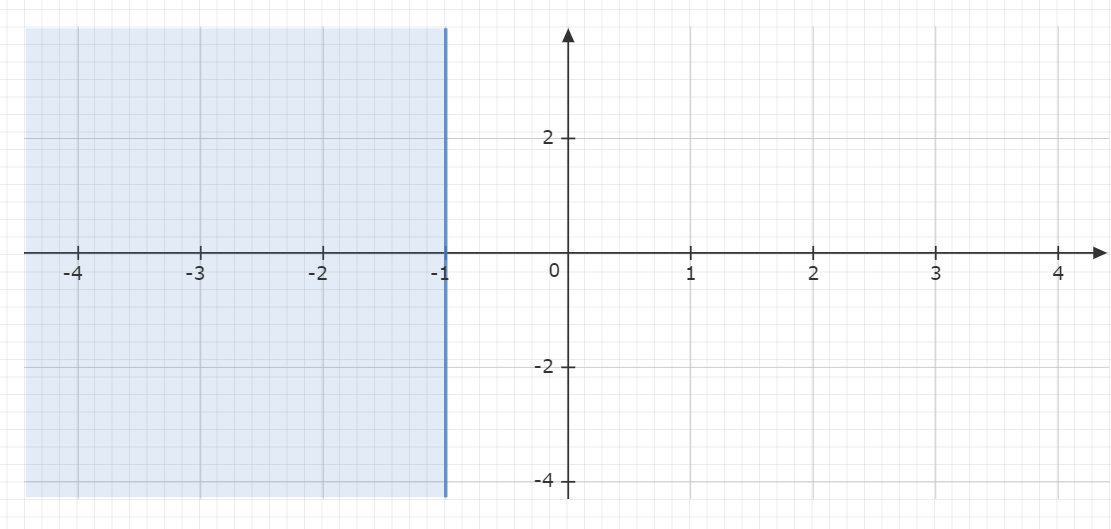
\includegraphics[width = 0.75 \textwidth]{images/1.png}
\end{center}



با این حال اگر فرض کنیم که بیش از دو قطب داشته باشیم، نمی‌توانیم لزوما چپ سو بودن را نتیجه بگیریم. یعنی ممکن است مثلا عبارت ما از دو طرف محدود باشد و یک قطب دیگر هم داشته باشیم که راست سو باشد،  وهمین باعث بشود که حالت از دو طرف محدود پیش بیاید. (و همچنان هم در انتگرال ناپذیر بودن خللی وارد نمی‌شود، زیرا به هر حال همچنان یک جزء x(t) انتگرال ناپذیر است)

یا حالت دیگر این است که یک قطب چپ‌سوی دیگر در سمت منفی‌تر داشته باشیم و در آن صورت ناحیه بالا مثلا از منفی ۲ شروع می‌شد و نه منفی ۱.


همه این موارد با فرض حقیقی بودن سیگنال بود. در صورت مختلط بودن سیگنال، امکان این وجود دارد که مزدوج قطب دیگر جزو قطب‌ها نباشد. با این حال همچنان با استدلالی مشابه استدلال بالا و این که همچنان عامل $-1$ در توان وجود دارد می‌توان به این نتیجه رسید که $Re(s)<-1$. اما باز‌هم مشابه بالا از آن جایی که در مورد این که قطب‌های دیگری هم وجود دارند یا نه مطلع نیستیم، نمی‌توانیم به طور قطع در مورد چپ‌سو بودن یا از دو طرف محدود بودن نظر بدهیم.


\item

با توجه به توضیحات بالا اگر سیگنال حقیقی و با دقیقا دو قطب باشد چپ سو است. در مورد سایر حالات در بالا به تفضیل توضیح داده شده است.
	
\end{enumerate}


در نهایت توجه کنید که عبارت $X(0)=8$
تنها می تواند در تعیین ضریب صورت تاثیر گذار باشد و برای مواردی که در سوال گفته شده، به طور مستقیم نقشی ندارد. اگر سوال می خواست که به طور دقیق تر خود $X(S)$ را مشخص کنیم آن گاه این عبارت هم تاثیر گذار می‌شد.


\section{سوال پنجم}

حل تحلیلی معادله:
$$
3 \ddot{x}(t)+30 \dot{x}(t)+63 x(t)=4 \dot{g}(t)+6 g(t)
$$

$$
x(0)=4, \dot{x}(0)=7
$$

و $g(t)=u(t)$

بر این اساس و براساس رابطه لاپلاس برای مشتق داریم:

$$3 \times (s^2X(s) - sx(0) - \dot{x}(0)) + 30 \times (sX(s)-x(0)) + 63 x(S) = 4 + \frac{6}{s}$$


$$3 \times (s^2X(s) - 4s - 7) + 30 \times (sX(s)-4) + 63 X(s) = 4 + \frac{6}{s}$$

با حل معادله برحسب $X(s)$ داریم:

$$
X(s)=\frac{12 s^{2}+145 s+6}{3 s\left(s^{2}+10 s+21\right)}
$$
$$
=\frac{12 s^{2}+145 s+6}{3 s(s+3)(s+7)}
$$
$$
\frac{107}{12 (s+3)}-\frac{421}{84 (s+7)}+\frac{2}{21 s}
$$

و ROC آن را هم با توجه به معادله دیفرانسیل بودن و این که عموما فرض کلی ODE ها صفر بودن وضعیت سیستم در منفی‌ بی‌نهایت است، سمت راست محور مختصات خواهد بود.

با تبدیل معکوس لاپلاس گرفتن داریم:

$$(\frac{107}{12} e^{-3t} - \frac{421}{84}e^{-7t} + \frac{2}{21})u(t) ; t>0$$

دلیل این که عبارت را راست‌سو گذاشتیم معادله دیفرانسیل بودن آن است. معمولا در سوالات مربوط به معادلات دیفرانسیل، هدف پیش‌بینی وضعیت سیستم بعد از آن است. به علاوه عبارتی که برای مشتق لاپلاس نوشته شده، از لاپلاس Unilateral یک طرفه که از $0$ تا $+\infty$ است بدست می‌آید و با لاپلاس رایج این درس که از $-\infty$ تا $+\infty$ است تفاوت دارد.

با این حال اگر فرض کنیم با لاپلاس Bilateral این درس محاسبه کنیم، عبارت‌های مربوط به شرایط اولیه از بین می‌روند (با فرض این که در منفی بی‌نهایت سیستم در حالت $0$ بوده باشد.) در این حالت،  معادلات به شکل زیر می‌شود



$$3 \times (s^2X(s)) + 30 \times (sX(s)) + 63 X(s) = 4 + \frac{6}{s}$$

$$X(s)= \frac{(2 (3 + 2 s))}{(3 s (21 + 10 s + s^2))}$$

$$= \frac{1}{6 (s+3)}-\frac{11}{42 (s+7)}+\frac{2}{21 s}$$


$$(\frac{e^{-3t}}{6} - \frac{11 e^{-7t}}{42} + \frac{2 e^{-t}}{21})u(t) ; t>0$$

همچنان چون معادلات دیفرانسیل معمولا با این فرض هستند که سیستم در قبل از لحظه صفر در حالت $0$ بوده است و ما هم برای منفی بی‌نهایت چنین فرضی کردیم، عبارت‌ $u(t)$ ضرب شده است.

\textbf{با این حال، جواب درست معادله دیفرانسیل، همان جواب قسمت اول است که به کمک لاپلاس Unilateral نوشته شده است. جواب دوم به طور کلی شرایط اولیه را نادیده گرفته است.}
\end{document}



